\chapter{Micro Controller Board Library}

\section{Introduzione}

La libreria \texttt{MicroControllerBoard} consente di comunicare con le schede a micro-controllore
sviluppate nella stazione radioastronomica di Medicina (Bologna)\footnote{Il protocollo di comunicazione 
\`e descritto in dettaglio nel documento interno IRA n.358/04 (F.Fiocchi, G.Macaferri, A.Oralti, M.Morsiani). 
Il firmware che controlla le schede \`e stato realizzato da Franco Fiocchi mentre dell'hardware se ne sono 
occupati Sandro Cattani ed Andrea Maccaferri.}.

In questo capitolo non ci occuperemo esclusivamente della libreria dal punto di vista software,
ma tratteremo anche aspetti di pi\`u basso livello e nascosti dalla libreria,  come il protocollo di comunicazione e l'architettura
hardware delle schede a microcontrollore. Lo scopo di questo documento \`e quindi anche quello di poter essere utilizzato
come riferimento per quanto concerne la comprensione dell'implementazione software del protocollo.


\section{Protocollo di Comunicazione\label{sec:protocollo}}
Per meglio comprendere le caratteristiche e la codifica del protocollo occorre chiarire la distinzione tra
un dispositivo definito \emph{master}\index{master} ed uno \emph{slave}\index{slave}, attraverso una definizione univoca:
\begin{itemize}
\item \emph{master}: dispositivo che invia ad un altro dispositivo un pacchetto di dati sul canale di comunicazione;
\item \emph{slave}: dispositivo che riconosce il pacchetto di dati a lui indirizzato e, se richiesto, manda
al dispositivo chiamante un pacchetto di dati in risposta.
\end{itemize}
Il protocollo sviluppato \`e del tipo \emph{multi-master}\index{multi-master}, in quanto permette la realizzazione di reti ad
architettura semplice, come quella del tipo \emph{master-slave}\index{master-slave}, oppure complessa come quella \emph{multi-master}
dove il controllo pu\`o essere ridondante o dove dispositivi diversi possono condividere le medesime risorse.

La trasmissione di pacchetti consistenti di dati posono mettere in difficolt\`a i dispositivi di elaborazione dotati di
micro-controllori, in quanto normalmente dotati di ristretti buffer di comunicazione. Nel protocollo \`e stato
quindi previsto un meccanismo per frammentare la comunicazione in pacchetti di dati pi\`u piccoli denominati
\emph{frames}\index{frames}.

I comandi e le risposte sono suddivisi in due gruppi principali:
\begin{itemize}
\item \emph{comandi estesi}\index{comandi!estesi}: per i quali, come si evince dal loro nome, la codifica \`e pi\`u lunga ed
\`e presente un campo \emph{checksum}\index{checksum}, utilizzato per controllare che la comunicazione tra due dispositivi
sia esente da errori di trasmissione\footnote{Il carattere di checksum si ottiene eseguendo la funzione logica EX-OR (OR esclusivo)
di tutti i suoi precedenti byte incluso quello di apertura della trasmissione.}.
\item \emph{comandi abbreviati}\index{comandi!abbreviati}: per i quali non \`e presente il controllo del \emph{checksum} e nemmeno
il carattere terminatore.
\end{itemize}
Entrambi i gruppi contengono i medesimi comandi (contraddistinti con identificativi diversi che ne determinano l'appartentenza),
elencati di seguito:
\begin{itemize}
\item \texttt{CMD\_INQUIRY}\index{comando!inquiry}: chiede allo slave di ritornare l'identificativo e 
l'esito dell'ultimo comando eseguito,
insieme alla data e all'ora di esecuzione. Pu\`o essere utilizzato, per esempio, dopo un comando indirizzato a tutti gli 
slave che non preveda la risopsta, al fine di conoscere l'esito di uno slave specifico. Se come indicativo dell'ultimo
comando eseguito, il dispositivo torna zero (0x00), significa che non ha ancora esegito alcuna operazione dal momento
dell'accensione. L'esecuzione di un comando INQUIRY non viene memorizzata dai dispositivi, quindi \texttt{CMD\_INQUIRY} non
compare mai come identificativo dell'ultimo comando eseguito.
\item \texttt{CMD\_RESET}\index{comando!reset}: forza lo slave a terminare ogni attivit\`a che ha in coda d'esecuzione ed a ricominiciare da
capo l'esecuzione del suo programma applicativo; questo equivale a riportare il dispositivo nella stessa condizione iniziale,
quando gli viene applicata l'alimentazione.
\item \texttt{CMD\_VERSION}\index{comando!version}: chiede allo slave di ritornare il codice identificativo. Il codice ritornato dipende dall'hardware
del dispositivo slave e dall'applicativo su di esso sviluppato. In generale \`e composto da tre sezioni riportanti un
identificativo della scheda (primi quattro caratteri), la versione del firmware (i due caratteri seguenti) e la relativa revisione
(ultimi due caratteri).
\item \texttt{CMD\_SAVE}\index{comando!save}: permette di salvare su memoria non volatile i parametri di configurazione dello slave;
questi dipendono dall'hardware del dispositivo e dall'applicativo su di esso sviluppato. I dati di configurazione sono le
impostazioni di default, ovvero quelle caricate al momento dell'alimentazione della scheda.
\item \texttt{CMD\_RESTORE}\index{comando!restore}: permette di recuperare dalla memoria non volatile i parametri di configurazione dello slave;
questi dipendono dall'hardware del dispositivo e dall'applicativo su di esso sviluppato. Dopo il recupero della configurazione,
il dispositivo slave esegue un reset a caldo in modo da rendere operativa la nuova configurazione, che utilizzer\`a tutte le volte
che verr\`a alimentato.
\item \texttt{CMD\_GET\_ADDR}\index{comando!get address}: chiede allo slave di ritornare il suo indirizzo di protocollo.
\item \texttt{CMD\_SET\_ADDR}\index{comando!set address}: comunica il nuovo indirizzo di protocollo che lo slave deve utilizzare; la riposta al comando
viene data col vecchio indirizzo, dopodich\`e il dispositivo riposnder\`a solo ai comandi inviati al nuovo indirizzo. 
L'impostazione viene persa se viene a mancare l'alimentazione allo slave; per salvarla in modo non volatile \`e 
necessario inviare allo slave (al suo nuovo indirizzo) un comando \texttt{CMD\_SAVE}.
\item \texttt{CMD\_GET\_TIME}\index{comando!get time}: chiede allo slave di ritornare la data e l'orario del suo orologio interno nella seguente
sequenza: secolo, anno, mese, giorno, ora, minuti, secondi e centesimi di secondo.
\item \texttt{CMD\_SET\_TIME}\index{comando!set time}: chiede allo slave di impostare l'orario e la data del suo orologio interno nella seguente
sequenza: secolo, anno, mese, giorno, ora, minuti, secondi e centesimi di secondo.
\item \texttt{CMD\_GET\_FRAME}\index{comando!get frame}: chiede allo slave di ritornare la dimensione massima del campo PARAMETER (per i comandi)
e DATA (per le risposte); questa dimensione dipende dall'hardware del dispositivo e dall'applicativo su di esso
sviluppato.
\item \texttt{CMD\_SET\_FRAME}\index{comando!set frame}: chiede allo slave di limitare la dimensione massima del campo PARAMETER (per i comandi)
e DATA (per le risposte); questa dimensione dipende dall'hardware del dispositivo e dall'applicativo su di esso sviluppato.
\item \texttt{CMD\_GET\_PORT}\index{comando!get port}: chiede allo slave di ritornare l'impostazione della porta, ovvero i parametri di configurazione
necessari a definire il funzionamento; una porta parallela, ad esempio, necessita la configurazione della direzione 
(ingresso/uscita) dei vari bit che costituiscono la parola.
\item \texttt{CMD\_SET\_PORT}\index{comando!set port}: chiede allo slave di modificare l'impostazione della porta, ovvero i parametri di configurazione
necessari a definire il funzionamento; una porta parallela, ad esempio, necessita la configurazione della direzione 
(ingresso/uscita) dei vari bit che costituiscono la parola.
\item \texttt{CMD\_GET\_DATA}\index{comando!get data}: chiede allo slave di ritornare i dati presenti sulla porta; per una porta parallela, ad esempio,
ritorna lo stato dei vari bit che costituiscono la parola.
\item \texttt{CMD\_SET\_DATA}\index{comando!set data}:  chiede allo slave di modificare i dati presenti sulla porta; per una porta parallela, ad esempio,
imposta lo stato dei vari bit che costituiscono la parola.
\end{itemize}
\`E possibile eseguire tutti i comandi appena elencati utilizzando la libreria \texttt{MicroControllerBoard}, la quale si occupa
anche della verifica della risposta ed eventualmente del controllo degli errori mediante checksum.

Per maggiori dettagli sul protocollo si veda~\cite{mcontroller-protocol}.


\section{Il controllo del Dewar e degli LNA}
Come gi\`a detto in precedenza, nella stazione radioastronomica di Medicina (BO)
sono state progettate e realizzate delle scheda a microcontrollore con le quali \`e possibile
dialogare utilizzando il protocollo descritto nella sezione~\ref{sec:protocollo}.
Su ciascun ricevitore vengono installate due di queste schede, una utilizzata per il controllo del \emph{dewar}\index{dewar}
e l'altra per il controllo degli LNA. Nelle sezioni che seguono \`e descritta in dettaglio l'architettura
di queste due schede.

\subsection{LNAs control board\label{sec:lna-section}}
La scheda ha una duplice funzione: alimentare gli LNA\index{LNA (Low Noise Amplifier)} 
(Low Noise Amplifier) dei feed e permettere la lettura
dei valori delle grandezze
$V_D$, $I_D$ e $V_G$ di ogni \emph{stadio}\index{stadio} degli LNA di ciascun feed, e per ogni \emph{canale}\index{canale}. La scheda 
\`e divisa in due sezioni, una per la \emph{polarizzazione}\index{polarizzazione} 
left e l'altra per la right (due canali), ed ogni sezione
pu\`o alimentare~5 LNA (5 stadi di amplificazione).

Le letture vengono fatte sulla porta AD24\index{porta!AD24}, ed ogni lettura consente di recuperare i valori delle grandezze
di 8 canali per volta (4 feed, 2 canali per feed). 
Per poter effettuare una lettura \`e necessario indicare
quali grandezze andare a leggere, e questo viene fatto andando a scrivere sulla porta DIO\index{porta!DIO}. 

Le porte di nostro interesse quindi sono due:
\begin{itemize}
\item DIO: \`e una porta a 16 bit accessibile in lettura/scrittura;
\item AD24: \`e una porta con 8 locazioni da 32 bit (4 byte per ogni locazione).
\end{itemize}
Iniziamo con la descrizione della porta AD24, schematizzata in figura~\ref{fig:AD24}.
Una lettura dalla porta AD24 fornisce quindi un dato composto da 32 byte (ogni locazione $AD8, \dots, AD15$
\`e composta da 4 byte). Dalla locazione AD8 sar\`a possibile leggere la grandezza di interesse per il 
canale left di uno dei seguenti feed: 0, 1, 8 o 9, mentre dalla locazione AD9 sar\`a possibile leggere
il valore del canale right per gli stessi feed, e cos\`i via per tutti gli altri feed sulla base dello schema
di figura~\ref{fig:AD24}. 
\begin{center}
\begin{figure}[!htbp]
        \begin{center}
        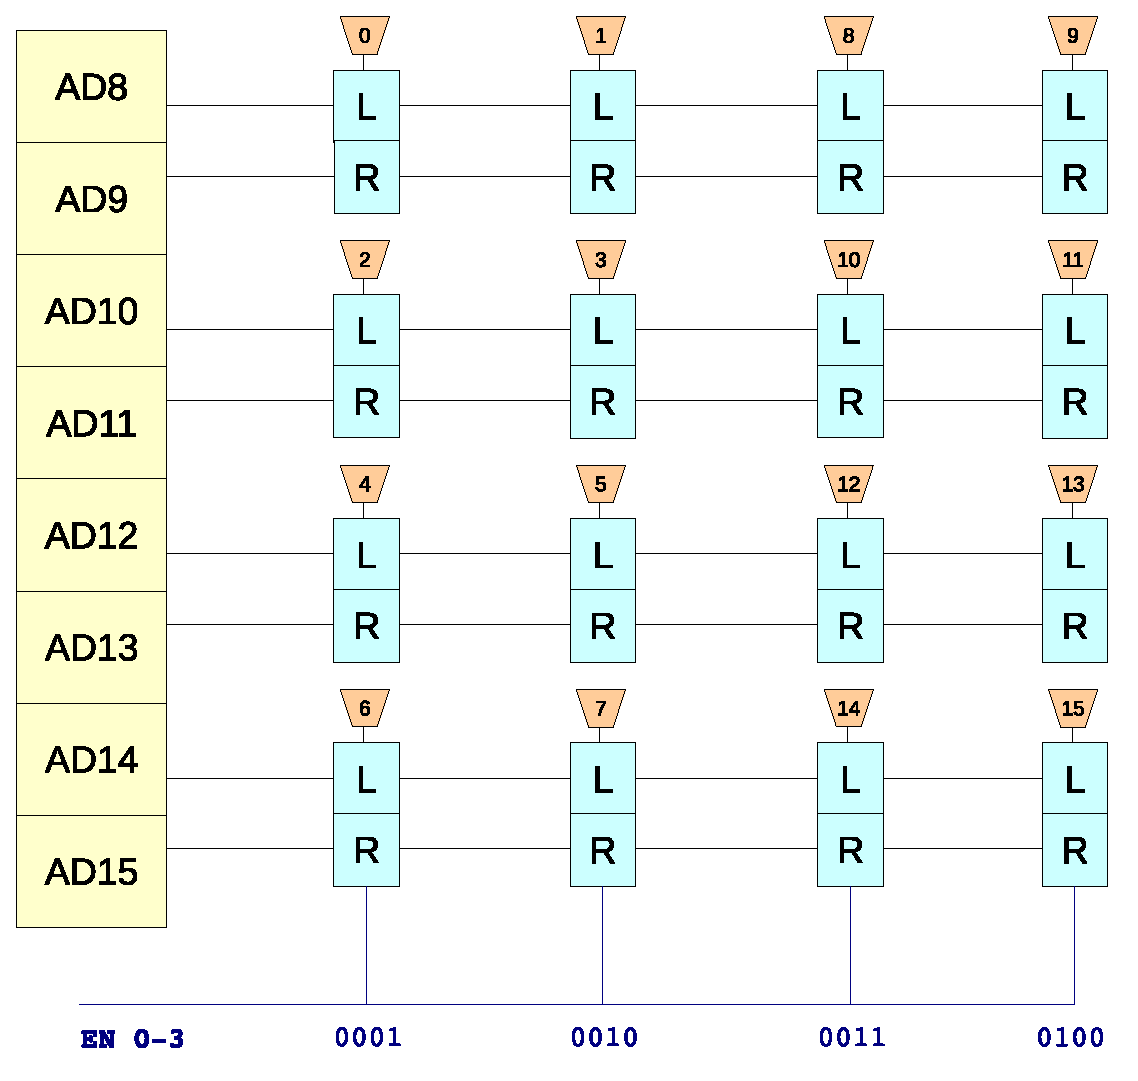
\includegraphics[width=11cm]{figure/AD24}
        \end{center}
        \figurecaption{Schema a blocchi della porta AD24}
         \label{fig:AD24}
\end{figure}
\end{center}
\`E possibile selezionare i feed su cui andare a leggere impostando sulla porta
DIO il valore di \texttt{EN 0-3}; come si vede in figura il valore \texttt{0001} di \texttt{EN 0-3} permette
di selezionare la prima colonna, il valore \texttt{0010} la seconda e cos\`i via per le altre due. La grandezza
da leggere invece dipende dal valore \texttt{AD 0-3} impostato nel DIO; questo permette di selezionare il valore di
$V_D$, $I_D$ o $V_G$ di uno dei cinque stadi degli LNA. La porta DIO \`e schematizzata in figura~\ref{fig:DIO}.
\begin{center}
\begin{figure}[!htbp]
        \begin{center}
        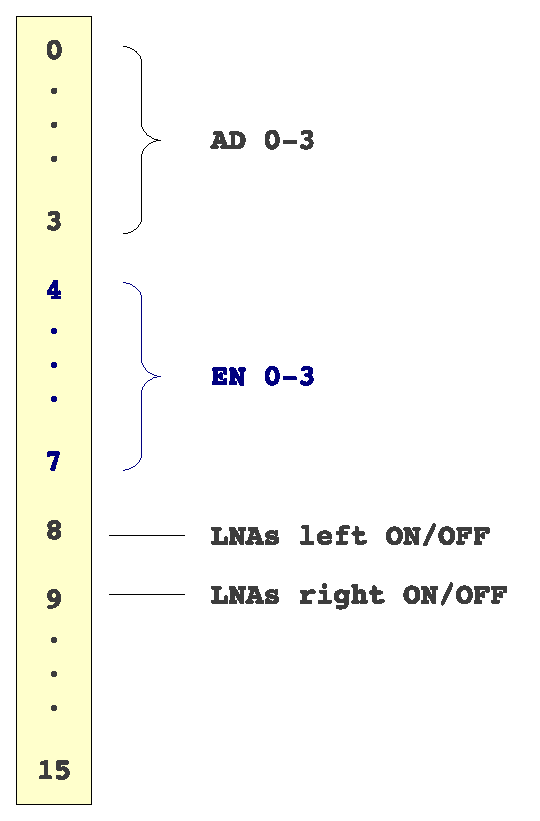
\includegraphics[width=5cm]{figure/DIO}
        \end{center}
        \figurecaption{Schema della porta DIO}
         \label{fig:DIO}
\end{figure}
\end{center}
Nella tabella~\ref{tab:AD03} sono indicati i valori di \texttt{AD 03} da impostare sulla porta DIO
per selezionare la grandezza da leggere.
\renewcommand\arraystretch{1.2}
\begin{table}[!htbp]
\begin{center}
\begin{tabular}{ c | c | p{4cm} }
\texttt{AD 0-3} & \textbf{Segnale} & \textbf{Stadio} \\
\hline 
\hline 
\texttt{0000} & $V_D$ & primo \\
\hline 
\texttt{0001} & $I_D$ & primo \\
\hline 
\texttt{0010} & $V_G$ & primo \\
\hline 
\texttt{0011} & $V_D$ & secondo \\
% \hline 
% \texttt{0100} & $I_D$ & secondo \\
% \hline 
% \texttt{0101} & $V_G$ & secondo \\
% \hline 
\dots & \dots & \dots \\
\hline
% \texttt{0110} & $V_D$ & terzo \\
% \hline 
% \texttt{0111} & $I_D$ & terzo \\
% \hline 
% \texttt{1000} & $V_G$ & terzo \\
% \hline 
% \texttt{1001} & $V_D$ & quarto \\
% \hline 
% \texttt{1010} & $I_D$ & quarto \\
% \hline 
% \texttt{1011} & $V_G$ & quarto \\
% \hline 
% \texttt{1100} & $V_D$ & quinto \\
% \hline 
% \texttt{1101} & $I_D$ & quinto \\
% \hline 
% \texttt{1110} & $V_G$ & quinto \\
% \hline 
\end{tabular}
\caption{Valori di \texttt{AD 0-3} per la selezione della grandezza da leggere}
\label{tab:AD03}
\end{center}
\end{table}

Supponiamo ad esempio di voler leggere gli 8 valori (4 feed, 2 canali per feed) di $V_G$ del terzo 
stadio dei feed 8, 10, 12 e 14. Il valore di \texttt{EN 0-3} sar\`a \texttt{0011} mentre il valore 
di \texttt{AD 0-3} sar\`a \texttt{1000}. Faremo allora due richieste: la prima (\texttt{SET\_DATA}\index{comando!set data}) 
ha lo scopo di configurare la porta DIO in modo da impostare i valori di 
\texttt{AD 0-3} e \texttt{EN 0-3}, mentre la seconda (\texttt{GET\_DATA}\index{comando!get data}) \`e la lettura della 
grandezza richiesta ($V_G$ del terzo stadio per i vari feed):
\begin{itemize}
\item \texttt{SET\_DATA}: avr\`a quattro \emph{parametri}\index{parametri}:
\begin{enumerate}
\item \textbf{data type}: unsigned da 8 bit
\item \textbf{port type}: DIO
\item \textbf{port number}: da 0 a 7 (8 bit, dall'indice 0 all'indice 7)
\item \textbf{value}: \texttt{10000011} (\texttt{AD 0-3} + \texttt{EN 0-3})
\end{enumerate}
\item \texttt{GET\_DATA}: avr\`a tre parametri\index{parametri}:
\begin{enumerate}
\item \textbf{data type}: 32 bit floating point
\item \textbf{port type}: AD24
\item \textbf{port number}: da 8 a 15
\end{enumerate}
\end{itemize}
Dopo aver dato il comando \texttt{SET\_DATA} \`e necessario attendere un \emph{tempo di guardia}\index{tempo di guardia} prima di
andare a leggere i valori con \texttt{GET\_DATA}, in modo da avere le uscite stabili; questo
tempo di guardia non deve essere inferiore ai $200$\,ms.

Il dato letto con il \texttt{GET\_DATA} \`e un 32 byte, che una volta scomposto in elementi da 4 byte ci fornisce
8 valori analogici di tensione, che andranno poi convertiti secondo opportune formule di trasformazione.


\subsection{Dewar Control Board}
Anche la scheda per il controllo del \emph{dewar}\index{dewar} ha una porta DIO ed una porta AD24, ma a differenza 
della scheda per il controllo degli LNA non \`e necessario scrivere sulla porta DIO prima di 
leggere dalla porta AD24, poich\`e non \`e possibile specificare quali grandezze leggere dalla porta
AD24; queste infatti non cambiano e sono le seguenti:
\begin{enumerate}
\item \texttt{AD08}: temperatura criogenica\index{temperatura!criogenica} numero 1;
\item \texttt{AD09}: temperatura criogenica numero 2;
\item \texttt{AD10}: pressione\index{pressione} all'interno del dewar;
\item \texttt{AD11}: temperatura criogenica numero 3;
\item \texttt{AD12}: temperatura criogenica numero 4;  
\item \texttt{AD13}: spare temperature\index{temperatura!spare};
\item \texttt{AD14}: vertex temperature{temperatura!vertex}\index{vertex};
\item \texttt{AD15}: spare temperature.
\end{enumerate}
I valori di tensione letti andranno poi convertiti tramite opportune formule in modo da ottenere i valori
nelle corrette unit\`a ingegneristiche (ad esempio in Kelvin o mbar).

Le porte ed i \emph{numeri di porta}\index{numeri di porta} descritti in questo documento sono relativi 
alle schede montate sul ricevitore
22 GHz multi-beam\index{ricevitore 22GHz} in funzione su SRT, ma le schede che verranno montate sui futuri ricevitori non dovrebbero
cambiare questa mappatura. I dettagli tecnici sulla scheda per il controllo degli LNA e su quella per
il controllo del dewar sono reperibili rispettivamente nei documenti~\cite{lna-controls}
e~\cite{dewar-controls}.

% Vediamo in questa sezione le principali operazioni che e
% del dewar. Indicare che i primi 16 bit possono essere scritti e letti, mentre i restanti 16 possono
% essere solo letti.
% \begin{enumerate}
% \item texttt{OUT\_00}: si pone il bit a 0 per selezionare l'oscillatore locale 1, mentre lo si
% pone ad 1 per selezionare l'oscillatore locale 2;
% \item texttt{OUT\_01}: libero
% \item texttt{OUT\_02}: libero
% \item texttt{OUT\_03}: 
% \item texttt{OUT\_04}:
% \item texttt{OUT\_05}:
% \item texttt{OUT\_06}:
% \item texttt{OUT\_07}:
% \item texttt{OUT\_08}:
% \item texttt{OUT\_09}:
% \item texttt{OUT\_10}:
% \item texttt{OUT\_11}: noise mark generator ON/OFF
% \item texttt{OUT\_12}: noise mark generator: external synchronous command enabled/disabled
% \item texttt{OUT\_13}: 
% \item texttt{OUT\_14}:
% \item texttt{OUT\_15}:
% \item texttt{IN\_00}: stato dell'oscillatore locale 1 (OL1). Quando il bit vale 1 allora OL1
% \`e selezionato;
% \item texttt{IN\_01}: stato dell'oscillatore locale 2 (OL2). Quando il bit vale 1 allora OL2
% \`e selezionato;
% \item texttt{IN\_02}: quando questo bit \`e a 1 OL2 \`e unlocked
% \item texttt{IN\_03}: remote/local
% \item texttt{IN\_04}: 
% \item texttt{IN\_05}: vacuum pump status
% \item texttt{IN\_06}: vacuum pump fault
% \item texttt{IN\_07}: vacuum valve status
% \item texttt{IN\_08}: 
% \item texttt{IN\_09}:
% \item texttt{IN\_10}:
% \item texttt{IN\_11}:
% \item texttt{IN\_12}:
% \item texttt{IN\_13}:
% \item texttt{IN\_14}:
% \item texttt{IN\_15}:
% \end{enumerate}


\section{Utilizzo della Libreria}
La \texttt{MicroControllerBoard} \`e una libreria thread-safe composta da~3 file: 
\emph{MicroControllerBoard.h} e \emph{MicroControllerBoard.cpp} nei quali viene rispettivamente
dichiarata e definita la classe \texttt{MicroControllerBoard}, ed il file \emph{MicroControllerBoardDef.h}
nel quale sono definiti tutti i parametri, come i \emph{tipi di dato}\index{tipo di dato}, le porte ed i numeri di porta.

Nel listato~\ref{lst:mcboard-getdata} \`e illustrato un breve esempio di utilizzo della
libreria, nel quale viene istanziato un oggetto MicroControllerBoard al fine di 
effettuare una richiesta \texttt{GET\_DATA}.
\lstset{language=C++}
\lstset{numbers=left,numberstyle={\scriptsize},stepnumber=1,firstnumber=1,numbersep=10pt}
\begin{lstlisting}[caption={[Esempio di utilizzo della libreria \texttt{MicroControllerBoard}]Esempio 
di utilizzo della libreria \texttt{MicroControllerBoard}},
label=lst:mcboard-getdata,mathescape]
#include "MicroControllerBoard.h"
#include <cstdlib>
using namespace IRA;

int main()
{
    // Definiamo i parametri IP e porta da passare al costruttore
    std::string IP("192.168.51.63"); // Indirizzo IP della scheda
    unsigned int port = 5002; // Numero di porta della connessione
    // Il vettore params conterra' i parametri del GET_DATA
    std::vector<BYTE> params;
    // Il data type e' un floating point a 32
    params.push_back(MCB_CMD_DATA_TYPE_F32);
    // La porta dalla quale leggere i dati e' la AD24
    params.push_back(MCB_PORT_TYPE_AD24); 
    // Vogliamo leggere un insieme di 8 dati floating point
    params.push_back(MCB_PORT_NUMBER_00_07);
    try {
        MicroControllerBoard mcb = MicroControllerBoard(IP, port);
        // Creiamo la connessione TCP/IP con la scheda
        mcb.openConnection();
        // Effettuiamo una richiesta GET_DATA
        mcb.send(MCB_CMD_GET_DATA, params);
        data = mcb.receive(); // Riceviamo i dati richiesti
        // Richiesta GET_DATA senza controllo checksum
        mcb.send(MCB_CMD_GET_DATA | MCB_CMD_TYPE_NOCHECKSUM, params);
        data = mcb.receive();
        mcb.closeConnection(); // Chiudiamo la connessione
    }
    catch(MicroControllerBoardEx& ex) {
        cout << ex.what() << endl;
        mcb.closeConnection();
        // ...
    }
    return 0;
}
\end{lstlisting}
\lstset{numbers=none}
Alle righe 11-17 viene creato il vettore di parametri che caratterizza la richiesta. I codici del
\textit{data type}, \textit{port type} e \textit{port number} sono definiti nel file
MicroControllerBoardDef.h, cos\`i come i codici dei comandi che vengono passati al metodo
\texttt{send} alle righe 23 e 26.

Quando nel metodo \texttt{send}\index{metodo!send} il codice di un comando viene messo in \texttt{or} con 
\texttt{MCB\_CMD\_TYPE\_NOCHECKSUM} (ad esempio, riga~26), significa che si sta effettuando
una comunicazione priva di controllo degli errori (nessun checksum).

Alle righe 24 e 27 viene invocato il metodo \texttt{receive}\index{metodo!receive}, il quale effettua tutti i 
possibili controlli sulla validit\`a della risposta:
\begin{itemize}
\item gli indirizzi del master\index{master} e dello slave\index{slave} della risposta devono coincidere con quelli della
richiesta;
\item il \emph{codice del comando}\index{codice del comando} deve essere valido;
\item risposta e richiesta devono avere lo stesso codice del comando;
\item l'identificativo (ID) della risposta deve essere lo stesso della richiesta;
\item il numero di parametri deve essere corretto;
\item il checksum\emph{checksum} (se richiesto) deve essere corretto.
\end{itemize}
